\documentclass{beamer}
\usepackage[backend=bibtex,style=numeric,sorting=none]{biblatex}
\usepackage{progressbar}
\usepackage[final]{listings}
\usepackage{graphicx}
\graphicspath{ {./images/} }

\addbibresource{main.bib}
\usetheme{AnnArbor}

\title{Container Security}
\subtitle{Bachelor's degree graduation project}
\author{Chih-Hsuan Yang}
\institute{National Sun Yat-sen University}
\date{\today\\v0.1}

\AtBeginSection[]{
    \begin{frame}
        \vfill
        \centering
        \begin{beamercolorbox}[sep=8pt,center,shadow=true,rounded=true]{title}
          \usebeamerfont{title}\insertsectionhead\par
        \end{beamercolorbox}
        \vfill
        \end{frame}
}

\definecolor{mygreen}{rgb}{0,0.6,0}
\definecolor{mygray}{rgb}{0.5,0.5,0.5}
\definecolor{mymauve}{rgb}{0.58,0,0.82}

% Code conf.
\lstset{ 
  backgroundcolor=\color{white},   % choose the background color; you must add \usepackage{color} or \usepackage{xcolor}; should come as last argument
  basicstyle=\ttfamily\footnotesize,% the size of the fonts that are used for the code
  breakatwhitespace=false,         % sets if automatic breaks should only happen at whitespace
  breaklines=true,                 % sets automatic line breaking
  captionpos=b,                    % sets the caption-position to bottom
  commentstyle=\color{mygreen},    % comment style
  deletekeywords={...},            % if you want to delete keywords from the given language
  escapeinside={\%*}{*)},          % if you want to add LaTeX within your code
  extendedchars=true,              % lets you use non-ASCII characters; for 8-bits encodings only, does not work with UTF-8
  frame=single,	                   % adds a frame around the code
  keepspaces=true,                 % keeps spaces in text, useful for keeping indentation of code (possibly needs columns=flexible)
  keywordstyle=\color{red},       % keyword style
  morekeywords={*,...},            % if you want to add more keywords to the set
  numbers=left,                    % where to put the line-numbers; possible values are (none, left, right)
  numbersep=5pt,                   % how far the line-numbers are from the code
  numberstyle=\tiny\color{mygray}, % the style that is used for the line-numbers
  rulecolor=\color{black},         % if not set, the frame-color may be changed on line-breaks within not-black text (e.g. comments (green here))
  showspaces=false,                % show spaces everywhere adding particular underscores; it overrides 'showstringspaces'
  showstringspaces=false,          % underline spaces within strings only
  showtabs=false,                  % show tabs within strings adding particular underscores
  stepnumber=1,                    % the step between two line-numbers. If it's 1, each line will be numbered
  stringstyle=\color{mymauve},     % string literal style
  tabsize=4,	                     % sets default tabsize to ˋ spaces
}


\begin{document}

\begin{frame}
    \titlepage
\end{frame}

\begin{frame}
    \frametitle{Outline}
    \tableofcontents
\end{frame}

% ======================Outcome============================
\section{Outcome}
\subsection{Expected Outcome}
\begin{frame}
    \frametitle{Medical cloud}
    \begin{itemize}
        \item Container
        \item Privacy, Security
        \item Load balanceability, Portability, Manageability
    \end{itemize}
\end{frame}

\subsection{Current Outcome}
\begin{frame}
    \frametitle{Current outcome}
    \begin{itemize}
        \item An easy container with Linux namespace.
    \end{itemize}
    \centering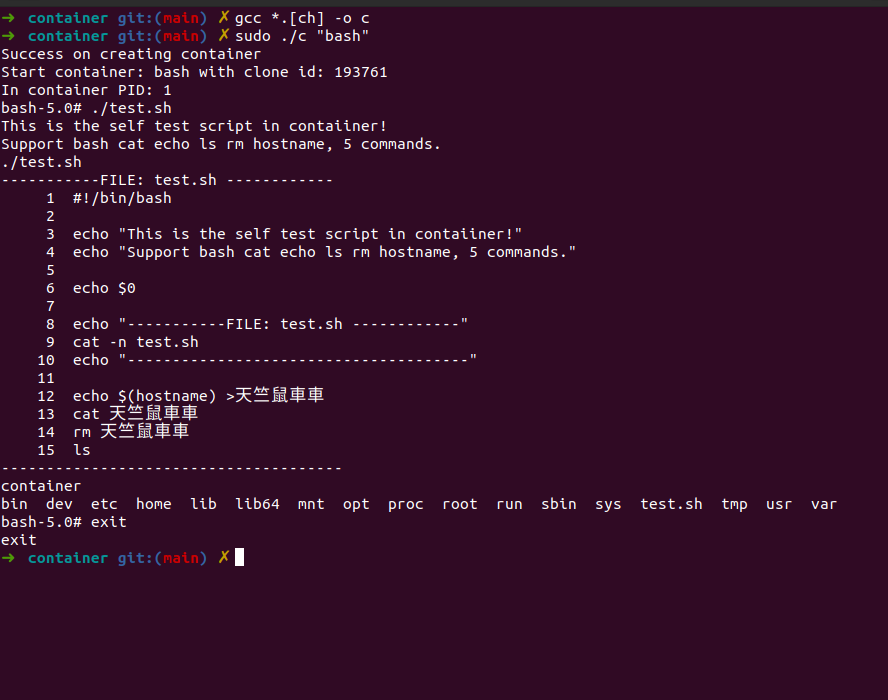
\includegraphics[width=1.0\textwidth]{cur_cont.png}
\end{frame}

\begin{frame}
    \frametitle{List of attack surface}
    \begin{itemize}
        \item Stack overflow?
        \item Kernel exploit
        \item cgroups with race condition
        \item namespace with wrong privileges
        \item Init.
    \end{itemize}
\end{frame}

% ======================FIXME============================

\section{FIXME}
\subsection{Linux feature}
\begin{frame}
    \frametitle{namespace}
    \begin{itemize}
        \item From Linux kernel 3.8
        \item System calls
              \begin{itemize}
                  \item clone, unshare, setns
              \end{itemize}
        \item Nested, scope
    \end{itemize}
    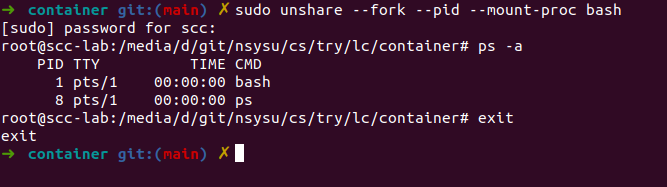
\includegraphics[width=\textwidth]{unshare_cmd.png}
\end{frame}

\begin{frame}
    \frametitle{namespace}
    \begin{itemize}
        \item 6 mechanisms
              \begin{itemize}
                  \item Mount, UTS, IPC, PID, NET, USER
              \end{itemize}
        \item ps: mount -t proc proc /proc
        \item $PID = 1$, the "init"\cite{docker_pid1}
              \begin{itemize}
                  \item SIGTERM, SIGKILL
                  \item The defunct
              \end{itemize}
    \end{itemize}
\end{frame}

\begin{frame}
    \frametitle{cgroups}
    \begin{itemize}
        \item Access controller
              \begin{itemize}
                  \item Resource limiting: CPU, Mem, IO\dots
                  \item Prioritization: CPU, IO\dots
                  \item Accounting: evaluate
                  \item Control: freeze, check, and resume
              \end{itemize}
        \item The OOM killer 4.19
              \begin{itemize}
                  \item Guarantee the integrity of the workload.
              \end{itemize}
    \end{itemize}
\end{frame}

\subsection{Exploit}
\begin{frame}
    \frametitle{Stack overflow}
    \begin{itemize}
        \item Default: 8MB
        \item The init of container, confused here.
    \end{itemize}
    \centering{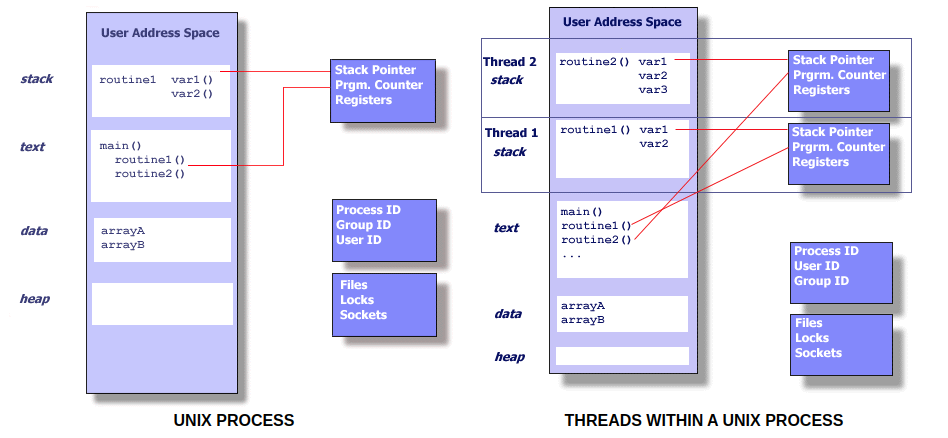
\includegraphics[width=\textwidth]{thread.png}}\cite{thread}
\end{frame}

% ======================Paper review============================

\section{Paper review}
\subsection{Papers}
\begin{frame}
    \frametitle{Have been read papers}
    \begin{itemize}
        \item Linux Kernel OS Local Root Exploit\cite{root_exploit}
        \item PINE: Optimizing Performance Isolation in Container Environments\cite{Optimizing}
        \item Study of Security Flaws in the Linux Kernel by Fuzzing\cite{Fuzzing}
    \end{itemize}
\end{frame}

\begin{frame}
    \frametitle{Linux Kernel OS Local Root Exploit}
    \begin{itemize}
        \item Dirty CoW
        \item race condition with mmap
        \item Counteract
              \begin{itemize}
                  \item Comparing the size of the binary against the size of the original binary\cite{root_exploit}
                  \item systemtap module
                  \item update \&\& upgrade
              \end{itemize}
    \end{itemize}
\end{frame}

\begin{frame}
    \frametitle{Optimizing Performance Isolation}
    \begin{beamerboxesrounded}{Microservices}
        \begin{itemize}
            \item latency-sensitive services
            \item throughput-first services
        \end{itemize}
        \centering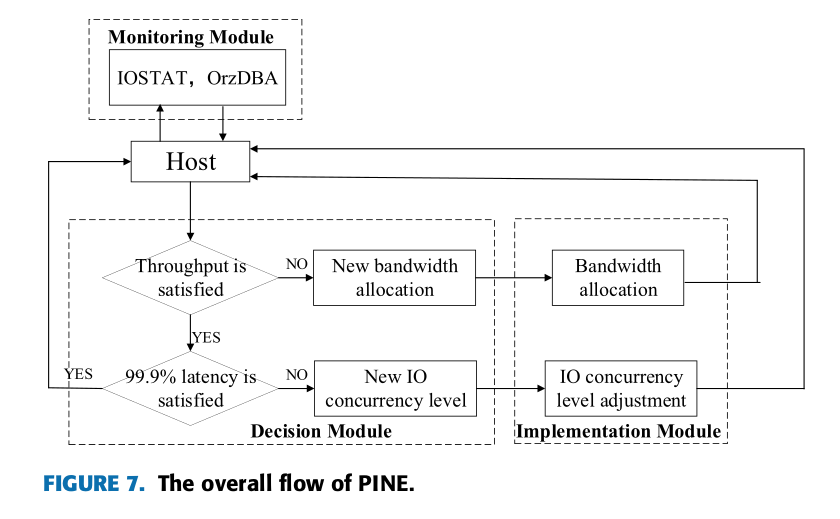
\includegraphics[width=0.7\textwidth]{PINE.png}\cite{Optimizing}
    \end{beamerboxesrounded}
\end{frame}

\begin{frame}
    \frametitle{Fuzzing}
    \begin{beamerboxesrounded}{Syzkaller}
        \begin{itemize}
            \item Stack overflow
                  \begin{itemize}
                      \item Canary
                      \item KSLR
                      \item Shadow stack
                  \end{itemize}
            \item Integer overflow
                  \begin{itemize}
                      \item Options to detected and SIGKILL
                  \end{itemize}
            \item Heap overflow
                  \begin{itemize}
                      \item Check size of the variable in comparison with the size copy\_to\_user, copy\_from\_user
                      \item Guard pages
                      \item Check functions and glibc's heap protections
                  \end{itemize}
        \end{itemize}
    \end{beamerboxesrounded}
\end{frame}

\begin{frame}
    \frametitle{Fuzzing}
    \begin{beamerboxesrounded}{Syzkaller}
        \begin{itemize}
            \item Format string injection
                  \begin{itemize}
                      \item Detect non-constant format string
                  \end{itemize}
            \item Kernel pointer leak
                  \begin{itemize}
                      \item Remove visibility for kernel symbols
                      \item Block the use of \%p
                  \end{itemize}
            \item Uninitialized variables
                  \begin{itemize}
                      \item RAII
                  \end{itemize}
            \item Use-after-free
                  \begin{itemize}
                      \item RAII too
                  \end{itemize}
        \end{itemize}
    \end{beamerboxesrounded}
\end{frame}

\subsection{Simple container}
\begin{frame}
    \frametitle{My container}
    \centering Code review
\end{frame}

\begin{frame}
    \frametitle{My container}
    \lstinputlisting[language=C, linerange={4-5}, firstnumber=4]{../../../try/lc/container/cont.h}
\end{frame}

\begin{frame}
    \frametitle{My container}
    \lstinputlisting[language=C, linerange={44-50, 52-54}, firstnumber=44]{../../../try/lc/container/cont.c}
    \lstinputlisting[language=C, linerange={38-42}, firstnumber=38]{../../../try/lc/container/cont.c}
\end{frame}

\begin{frame}
    \frametitle{My container}
    \lstinputlisting[language=C, linerange={25-29, 31-33, 35-36}, firstnumber=25]{../../../try/lc/container/cont.c}
    \lstinputlisting[language=C, linerange={15-20, 22-23}, firstnumber=15]{../../../try/lc/container/cont.c}
\end{frame}

% ======================Current progress============================

\section{Current progress}
\begin{frame}
    \frametitle{Application of MOST}
    \begin{itemize}
        \item \makebox[3cm]{Papers: \hfill} \progressbar[width=5cm,heightr=1,filledcolor=red,
                  emptycolor=blue!30]{1} 1.0
        \item \makebox[3cm]{FIXME: \hfill} \progressbar[width=5cm,heightr=1,filledcolor=red,
                  emptycolor=blue!30]{0.308} 0.308
        \item \makebox[3cm]{Pages: \hfill} \progressbar[width=5cm,heightr=1,filledcolor=red,
                  emptycolor=blue!30]{0.38} 0.380
        \item \makebox[3cm]{My Exp.: \hfill} \progressbar[width=5cm,heightr=1,filledcolor=red,
                  emptycolor=blue!30]{0.7} Maybe\dots
    \end{itemize}
\end{frame}

\begin{frame}
    \frametitle{Demo}
    \centering Live demo.
\end{frame}

\begin{frame}
    \frametitle{List of attack surface}
    \begin{itemize}
        \item Stack overflow?
        \item Kernel exploit
        \item cgroups with race condition
        \item namespace with wrong privileges
        \item Init.
    \end{itemize}
\end{frame}

\section{Reference}
\begin{frame}[t, allowframebreaks]
    \frametitle{References}
    \printbibliography
\end{frame}

\end{document}